\documentclass[a4paper]{scrartcl}

% font/encoding packages
\usepackage[utf8]{inputenc}
\usepackage[T1]{fontenc}
\usepackage{lmodern}
\usepackage[ngerman]{babel}
\usepackage[ngerman=ngerman-x-latest]{hyphsubst}

\usepackage{amsmath, amssymb, amsfonts, amsthm}
\usepackage{array}
\usepackage{stmaryrd}
\usepackage{marvosym}
\allowdisplaybreaks
\usepackage[output-decimal-marker={,}]{siunitx}
\usepackage[shortlabels]{enumitem}
\usepackage[section]{placeins}
\usepackage{float}
\usepackage{units}
\usepackage{listings}
\usepackage{pgfplots}
\pgfplotsset{compat=1.12}
\usepackage[hyphens]{url}
\usepackage{hyperref}
\usepackage{pdflscape}

\usepackage{tikz}
\usetikzlibrary{arrows,automata}
\usepackage{verbatim}

%\usepackage[newfloat]{minted}

\lstset{
    language=Python,
    numbers=left,
    frame=single,
    basicstyle=\footnotesize\ttfamily,
    otherkeywords={with,as},
}

\newtheorem*{behaupt}{Behauptung}
\newcommand{\gdw}{\Leftrightarrow}

\usepackage{fancyhdr}
\pagestyle{fancy}

\def \blattnr {7}

\lhead{GWV - Blatt {\blattnr}}
\rhead{Billis, Braun, Knapperzbusch, Nikolaisen}
\cfoot{\thepage}


\title{Grundlagen der Wissensverarbeitung}
\subtitle{Blatt {\blattnr} Hausaufgaben}
\author{
    Fabian Billis (6720351) \\
    Lennart Braun (6523742), \\
    Maximilian Knapperzbusch (6535090) \\
    Laurens Nikolaisen (6527179) \\
}
\date{zum 30. November 2015}

\begin{document}
\maketitle

\section*{Exercise \blattnr.2: CSI Stellingen}

\section*{Exercise \blattnr.3: Diagnosis}
	\begin{enumerate}
		\item
		\textbf{Assumables} \\
		\begin{align*}
			gardener_{worked} \\
			butler_{worked} \\
		\end{align*}
		
		\textbf{Rules}
		\begin{align*}
			gardener_{worked} &\leftarrow gdirtyhands \\
			butler_{worked} &\leftarrow bdirtyhands \\
		\end{align*}
		
		\textbf{Integrity Constraints}
		\begin{align*}
			false &\leftarrow gardener_{worked} \\
			false &\leftarrow butler_{worked} \\
		\end{align*}
		
		\textbf{Oberservations}
		\begin{align*}
			gdirtyhands &\leftarrow false \\
			bdirtyhands &\leftarrow true \\
		\end{align*}

		\item
		\textbf{Rules} \\
		\begin{align*}
		battery_{on} &\leftarrow battery_{ok}\\
		fuel \, tank_{on} &\leftarrow fuel \, tank_{ok}\\
		starter_{on} &\leftarrow starter_{ok} \wedge ignition \, key_{ok}\\
		ignition \, key_{on} &\leftarrow ignition \, key_{ok} \wedge electronic \, fuel \, regulation_{ok} \wedge battery_{ok} \\
		electronic \, fuel \, regulation_{on} &\leftarrow electronic \, fuel \, regulation_{ok} \wedge battery_{ok} \wedge ignition \, key_{ok} \\
		engine_{on} &\leftarrow engine_{ok} \wedge starter_{ok} \wedge filter_{ok}\\
		filter_{on} &\leftarrow filter_{ok} \wedge fuel pump_{ok} \wedge fuel tank_{ok} \\
		fuel pump_{on} &\leftarrow fuel pump_{ok} \wedge fuel \, tank_{ok} \wedge electronic \, fuel \, regulation_{ok}\\
		\end{align*}
		
		
		
		
		
		\textbf{Assumables} \\
		$
		battery_{ok}\\
		fuel \, tank_{ok} \\
		starter_{ok}\\
		ignition \, key_{ok}\\
		electronic \, fuel \, regulation_{ok}\\
		engine_{ok}\\
		filter_{ok}\\
		fuel pump_{ok}\\
		$
		
		\newpage	    
		
		\textbf{Integrity Constraints} \\
		$
		battery_{on} : battery_{off}\\
		fuel \, tank_{on} : fuel \, tank_{off} \\
		starter_{on} : starter_{off}\\
		ignition \, key_{on} : ignition \, key_{off}\\
		electronic \, fuel \, regulation_{on} : electronic \, fuel \, regulation_{off} \\
		engine_{on} : engine_{off}\\
		filter_{on} : filter_{off}\\
		fuel pump_{on} : fuel pump_{off}\\
		$	    
		
		Im Folgenden seien die Ableitungen der Regeln als Baumdiagramm dargestellt. Von diesen lässt sich dann relativ leicht eine (minimale) Diagnose erstellen. Im Bild wurden für die einzelnen Komponenten Abkürzungen verwendet:
		
		$
		battery : bat\\
		fuel \, tank_ : ft \\
		starter : st\}\\
		ignition \, key_{on} : ign\\
		electronic \, fuel \, regulation_{on} : elf\\
		engine_{on} : en\\
		filter_{on} : fil\\
		fuel pump_{on} : fp\\
		$
		
		
		
		%\begin{landscape}
		%	\begin{figure}[ht]
		%		\centering
		%		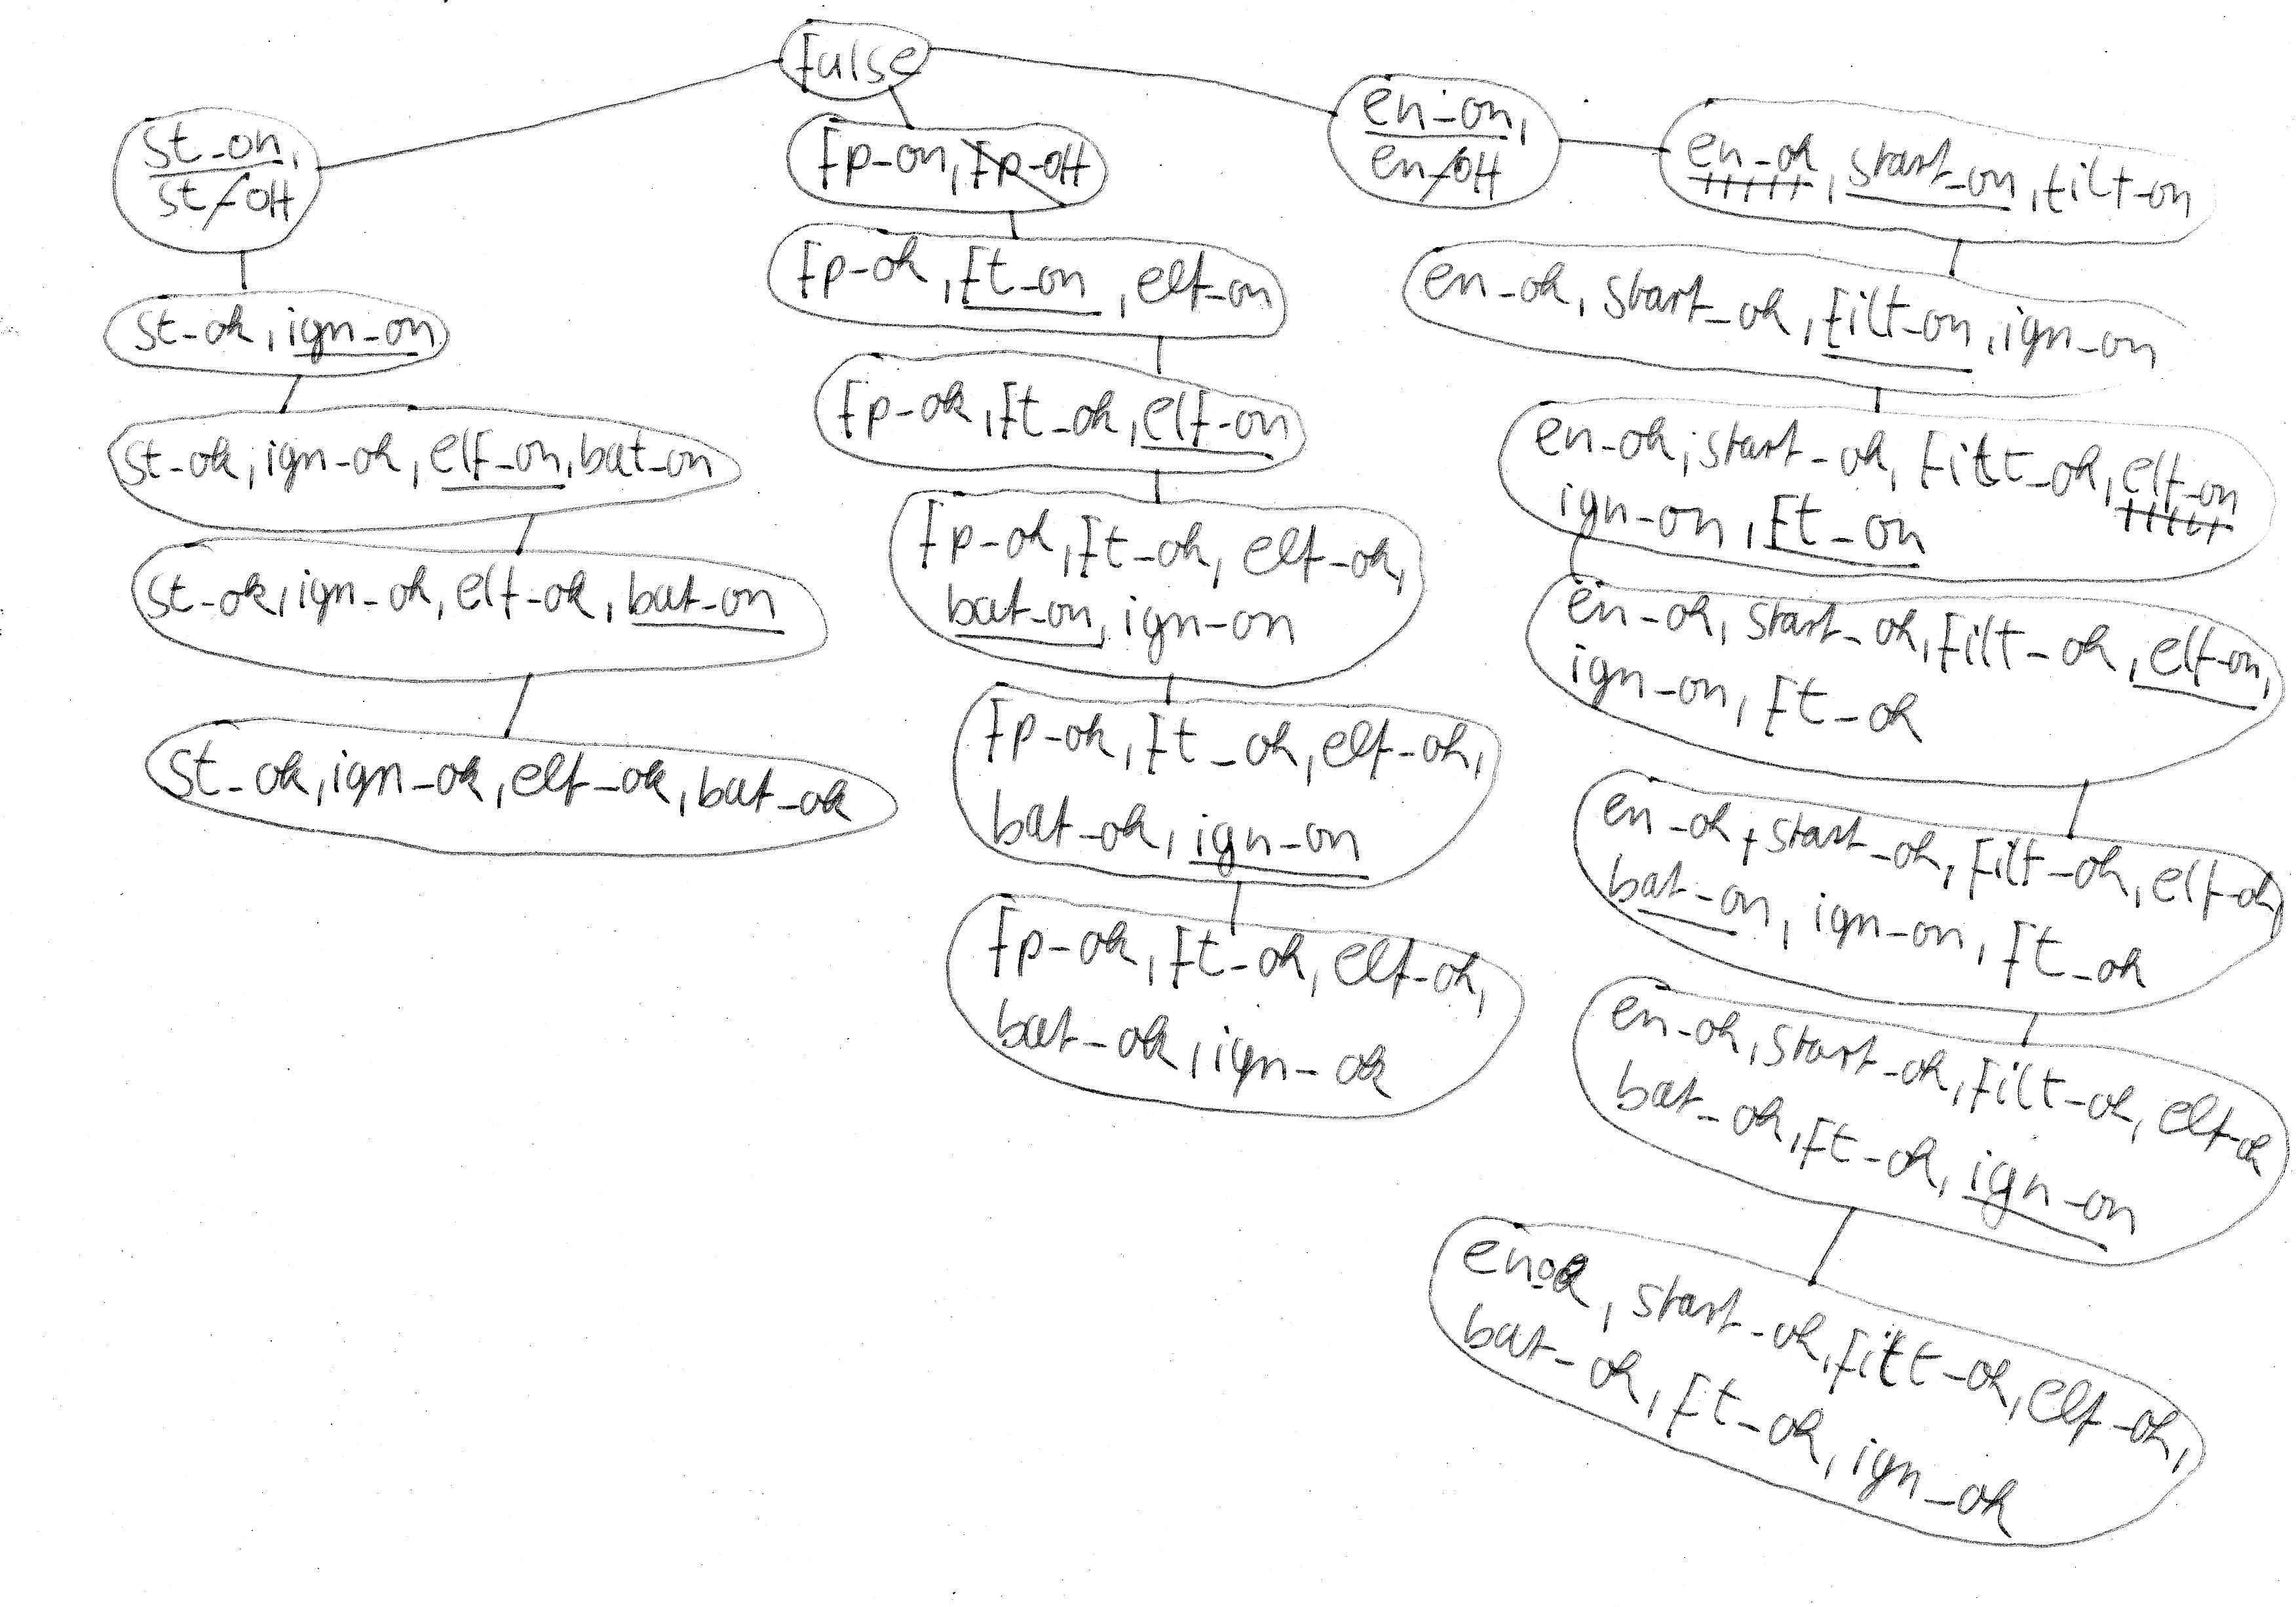
\includegraphics[width=1.5\textwidth]{baum.jpg}
		%		\caption{um 30 Grad gedreht}
		%		\label{fig1}
		%	\end{figure}
		

		%\end{landscape} 
		
		
		
		\textbf{Diagnosis}
			\begin{itemize}
				\item No noises: $starter \vee fuel \, pump \vee engine \rightarrow starter_{ok} \wedge fuel \, pump_{ok} \wedge  fuel \, tank_{ok} \wedge ignition \, key_{ok} \wedge electronic \, fuel \, regulation_{ok} \wedge  battery_{ok} \wedge filter_{ok} $ Alle Komponenten könnten kaputt sein, da die drei potenziell defekten Teile insgesamt mit allen anderen im Auto existierenden Bauteilen in direkter bzw. indirekter Verbindung stehen. Es ist nicht möglich das Problem einzugrenzen. Anders gesagt: Einer dieser Komponenten ist also nicht "`ok"' und somit wird die gesamte Struktur im Baum zu \textit{false} ausgewertet.
				
				\item Only noise 1
				
				\item Only noise 2
				
				\item Noise 1 and 2 but not noise 3
			\end{itemize}
		
		
%				battery_{on} &\leftarrow battery_{ok}\\
%				fuel \, tank_{on} &\leftarrow fuel \, tank_{ok}\\
%				starter_{on} &\leftarrow starter_{ok} \wedge ignition \, key_{ok}\\
%				ignition \, key_{on} &\leftarrow ignition \, key_{ok} \wedge electronic \, fuel \, regulation_{ok} \wedge battery_{ok} \\
%				electronic \, fuel \, regulation_{on} &\leftarrow electronic \, fuel \, regulation_{ok} \wedge battery_{ok} \wedge ignition \, key_{ok} \\
%				engine_{on} &\leftarrow engine_{ok} \wedge starter_{ok} \wedge filter_{ok}\\
%				filter_{on} &\leftarrow filter_{ok} \wedge fuel pump_{ok} \wedge fuel tank_{ok} \\
%				fuel pump_{on} &\leftarrow fuel pump_{ok} \wedge fuel \, tank_{ok} \wedge electronic \, fuel \, regulation_{ok}\\
		
		%Nennt man das so? 
	\end{enumerate}


\end{document}
